\begin{figure}[h]
    \centering
    \setlength{\resLen}{1.5in}
    \addtolength{\tabcolsep}{3pt}
    \begin{tabular}{ccc}
        & Forward & Backward\\
        \includegraphics[height=\resLen]{waveoptics/particle/aniso_z.jpg}
        & \multicolumn{2}{c}{\includegraphics[height=\resLen]{waveoptics/pfunc/aniso_z.jpg}}
        \\
        \includegraphics[height=\resLen]{waveoptics/particle/aniso_y.jpg}
        & \multicolumn{2}{c}{\includegraphics[height=\resLen]{waveoptics/pfunc/aniso_y.jpg}}
        \\
        \textbf{(a)} Incident direction & \multicolumn{2}{c}{\textbf{(b)} Phase function slice}
    \end{tabular}
    \caption[Visualizations of phase function]{\label{fig:waveoptics:aniso1}
        \textbf{Visualizations of slices $\phase(\dwi,\cdot)$ of a phase function} for two incident directions~$\dwi$ at $\lambda = 700\text{nm}$.
        This phase function is computed using a configuration where 100 particles with radii 500nm follow an anisotropic Gaussian distribution.
    }
\end{figure}
